% !TeX encoding = UTF-8

% 载入 SJTUThesis 模版
\documentclass[type=bachelor]{sjtuthesis}
% 选项
%   type=[doctor|master|bachelor],     % 可选(默认:master),论文类型
%   zihao=[-4|5],                      % 可选(默认:-4),正文字号大小
%   lang=[zh|en|de|ja],                % 可选(默认:zh),论文的主要语言
%   review,                            % 可选(默认:关闭),盲审模式
%   [twoside|oneside],                 % 可选(默认:twoside),双页或单页边距模式
%   [openright|openany],               % 可选(默认:openright),奇数页或任意页开始新章
%   math-style=[ISO|TeX],              % 可选 (默认:ISO),数学符号样式

% 论文基本配置,加载宏包等全局配置
% !TEX root = ./main.tex

\sjtusetup{
  %
  %******************************
  % 注意:
  %   1. 配置里面不要出现空行
  %   2. 不需要的配置信息可以删除
  %******************************
  %
  % 信息录入
  %
  info = {%
    %
    % 标题
    %
    zh / title           = {相对姿态测量下的多刚体姿态同步研究},
    en / title           = {Attitude Consensus of Multiple Rigid Bodies Based on Relative Attitude Measurement},
    %
    % 标题页标题
    %   可使用“\\”命令手动控制换行
    %
    % zh / display-title   = {上海交通大学学位论文\\ \LaTeX{} 模板示例文档},
    % en / display-title   = {A Sample Document \\ for \LaTeX-based SJTU Thesis Template},
    %
    % 关键词
    %
    zh / keywords        = {上海交大, 饮水思源, 爱国荣校},
    en / keywords        = {SJTU, master thesis, XeTeX/LaTeX template},
    %
    % 姓名
    %
    zh / author          = {周俊宇},
    en / author          = {Junyu Zhou},
    %
    % 指导教师
    %
    zh / supervisor      = {李贤伟教授},
    en / supervisor      = {Prof. Xianwei Li},
    %
    % 副指导教师
    %
    % assoc-supervisor  = {某某教授},
    % assoc-supervisor* = {Prof. Uom Uom},
    %
    % 学号
    %
    id              = {520021911029},
    %
    % 学位
    %   本科生不需要填写
    %
    zh / degree          = {学士},
    en / degree          = {Bachelor of Engineering},
    %
    % 专业
    %
    zh / major           = {自动化},
    en / major           = {A Very Important Major},
    %
    % 所属院系
    %
    zh / department      = {电子信息与电气工程学院},
    en / department      = {School of Electronic Information and Electric Engineering},
    %
    % 答辩日期
    %   使用 ISO 格式 (yyyy-mm-dd);默认为当前时间
    %
    % date                 = {2023-05-18},
    %
    % 标题页显示日期
    %   覆盖对应标题页的日期显示,原样输出
    %
    % zh / display-date    = {2023 年 5 月},
    %
    % 资助基金
    %
    % zh / fund  = {
    %                {国家 973 项目 (No. 2025CB000000)},
    %                {国家自然科学基金 (No. 81120250000)},
    %              },
    % en / fund  = {
    %                {National Basic Research Program of China (Grant No. 2025CB000000)},
    %                {National Natural Science Foundation of China (Grant No. 81120250000)},
    %              },
  },
  %
  % 风格设置
  %
  style = {%
    %
    % 论文标题页 logo 颜色 (red/blue/black)
    %
    % title-logo-color = black,
  },
  %
  % 名称设置
  %
  name = {
    % bib             = {References},
    % ack             = {谢\hspace{\ccwd}辞},
    % achv            = {攻读学位期间完成的论文},
  },
}

% 使用 BibLaTeX 处理参考文献
%   biblatex-gb7714-2015 常用选项
%     gbnamefmt=lowercase     姓名大小写由输入信息确定
%     gbpub=false             禁用出版信息缺失处理
\usepackage[backend=biber,style=gb7714-2015]{biblatex}
% 文献表字体
% \renewcommand{\bibfont}{\zihao{5}\fixedlineskip{15.6bp}}
% 文献表条目间的间距
\setlength{\bibitemsep}{0pt}
% 导入参考文献数据库
\addbibresource{refs.bib}

% 脚注格式
\usepackage[perpage,bottom,hang]{footmisc}

% 定义图片文件目录与扩展名
\graphicspath{{figures/}}
\DeclareGraphicsExtensions{.pdf,.eps,.png,.jpg,.jpeg}

% 确定浮动对象的位置,可以使用 [H],强制将浮动对象放到这里(可能效果很差)
% \usepackage{float}

% 固定宽度的表格
% \usepackage{tabularx}

% 使用三线表:toprule,midrule,bottomrule。
\usepackage{booktabs}

% 表格中支持跨行
\usepackage{multirow}

% 表格中数字按小数点对齐
\usepackage{dcolumn}
\newcolumntype{d}[1]{D{.}{.}{#1}}

% 使用长表格
\usepackage{longtable}

% 附带脚注的表格
\usepackage{threeparttable}

% 附带脚注的长表格
\usepackage{threeparttablex}

% 算法环境宏包
\usepackage[ruled,vlined,linesnumbered]{algorithm2e}
% \usepackage{algorithm, algorithmicx, algpseudocode}

% 代码环境宏包
\usepackage{listings}
\lstdefinestyle{lstStyleCode}{%
  aboveskip         = \medskipamount,
  belowskip         = \medskipamount,
  basicstyle        = \ttfamily\zihao{6},
  commentstyle      = \slshape\color{black!60},
  stringstyle       = \color{green!40!black!100},
  keywordstyle      = \bfseries\color{blue!50!black},
  extendedchars     = false,
  upquote           = true,
  tabsize           = 2,
  showstringspaces  = false,
  xleftmargin       = 1em,
  xrightmargin      = 1em,
  breaklines        = false,
  framexleftmargin  = 1em,
  framexrightmargin = 1em,
  backgroundcolor   = \color{gray!10},
  columns           = flexible,
  keepspaces        = true,
  texcl             = true,
  mathescape        = true
}
\lstnewenvironment{codeblock}[1][]{%
  \lstset{style=lstStyleCode,#1}}{}

% 直立体数学符号
\providecommand{\dd}{\mathop{}\!\mathrm{d}}
\providecommand{\ee}{\mathrm{e}}
\providecommand{\ii}{\mathrm{i}}
\providecommand{\jj}{\mathrm{j}}

% 国际单位制宏包
\usepackage{siunitx}

% 定理环境宏包
\usepackage{ntheorem}
% \usepackage{amsthm}

% 绘图宏包
\usepackage{tikz}
\usetikzlibrary{arrows.meta, shapes.geometric}

% 数据图表宏包
\usepackage{pgfplots}
\pgfplotsset{compat=newest}

% 一些文档中用到的 logo
\usepackage{hologo}
\providecommand{\XeTeX}{\hologo{XeTeX}}
\providecommand{\BibLaTeX}{\textsc{Bib}\LaTeX}

% 借用 ltxdoc 里面的几个命令方便写文档
\DeclareRobustCommand\cs[1]{\texttt{\char`\\#1}}
\providecommand\pkg[1]{{\sffamily#1}}

% hyperref 宏包在最后调用
\usepackage{hyperref}

% E-mail
\providecommand{\email}[1]{\href{mailto:#1}{\urlstyle{tt}\nolinkurl{#1}}}


\begin{document}

%TC:ignore

% 标题页
\maketitle

% 原创性声明及使用授权书
\copyrightpage
% 插入外置原创性声明及使用授权书
% 此时必须在导言区使用 \usepackage{pdfpages}
% \copyrightpage[scans/sample-copyright.pdf]

% 前置部分
\frontmatter

% 摘要
% !TEX root = ../main.tex

\begin{abstract}[zh]
  中文摘要应该将学位论文的内容要点简短明了地表达出来,应该包含论文中的基本信息,
  体现科研工作的核心思想。摘要内容应涉及本项科研工作的目的和意义、研究方法、研究
  成果、结论及意义。注意突出学位论文中具有创新性的成果和新见解的部分。摘要中不宜
  使用公式、化学结构式、图表和非公知公用的符号和术语,不标注引用文献编号。硕士学
  位论文中文摘要字数为 500 字左右,博士学位论文中文摘要字数为 800 字左右。英文摘
  要内容应与中文摘要内容一致。

  摘要页的下方注明本文的关键词(4 \textasciitilde{} 6个)。
\end{abstract}

\begin{abstract}[en]
  Shanghai Jiao Tong University (SJTU) is a key university in China. SJTU was
  founded in 1896. It is one of the oldest universities in China. The University
  has nurtured large numbers of outstanding figures include JIANG Zemin, DING
  Guangen, QIAN Xuesen, Wu Wenjun, WANG An, etc.

  SJTU has beautiful campuses, Bao Zhaolong Library, Various laboratories. It
  has been actively involved in international academic exchange programs. It is
  the center of CERNet in east China region, through computer networks, SJTU has
  faster and closer connection with the world.
\end{abstract}


% 目录
\tableofcontents
% 插图索引
\listoffigures*
% 表格索引
\listoftables*
% 算法索引
\listofalgorithms*

% 符号对照表
% !TEX root = ../main.tex

\begin{nomenclature*}
\label{chap:symb}

\begin{longtable}{rl}
  $\epsilon$  & 介电常数  \\  
  $\mu$       & 磁导率    \\
  $\epsilon$  & 介电常数  \\
  $\mu$       & 磁导率    \\
  $\epsilon$  & 介电常数  \\
  $\mu$       & 磁导率    \\
  $\epsilon$  & 介电常数  \\
  $\mu$       & 磁导率    \\
  $\epsilon$  & 介电常数  \\
  $\mu$       & 磁导率    \\
  $\epsilon$  & 介电常数  \\
  $\mu$       & 磁导率    \\
  $\epsilon$  & 介电常数  \\
  $\mu$       & 磁导率    \\
  $\epsilon$  & 介电常数  \\
  $\mu$       & 磁导率    \\
  $\epsilon$  & 介电常数  \\
  $\mu$       & 磁导率    \\
  $\epsilon$  & 介电常数  \\
  $\mu$       & 磁导率    \\
  $\epsilon$  & 介电常数  \\
  $\mu$       & 磁导率    \\
  $\epsilon$  & 介电常数  \\
  $\mu$       & 磁导率    \\
  $\epsilon$  & 介电常数  \\
  $\mu$       & 磁导率    \\
  $\epsilon$  & 介电常数  \\
  $\mu$       & 磁导率    \\
  $\epsilon$  & 介电常数  \\
  $\mu$       & 磁导率    \\
  $\epsilon$  & 介电常数  \\
  $\mu$       & 磁导率    \\
  $\epsilon$  & 介电常数  \\
  $\mu$       & 磁导率    \\
  $\epsilon$  & 介电常数  \\
  $\mu$       & 磁导率    \\
  $\epsilon$  & 介电常数  \\
  $\mu$       & 磁导率    \\
  $\epsilon$  & 介电常数  \\
  $\mu$       & 磁导率    \\
  $\epsilon$  & 介电常数  \\
  $\mu$       & 磁导率    \\
  $\epsilon$  & 介电常数  \\
  $\mu$       & 磁导率    \\
  $\epsilon$  & 介电常数  \\
  $\mu$       & 磁导率    \\
  $\epsilon$  & 介电常数  \\
  $\mu$       & 磁导率    \\
  $\epsilon$  & 介电常数  \\
  $\mu$       & 磁导率    \\
  $\epsilon$  & 介电常数  \\
  $\mu$       & 磁导率    \\
  $\epsilon$  & 介电常数  \\
  $\mu$       & 磁导率    \\
\end{longtable}

\end{nomenclature*}


%TC:endignore

% 主体部分
\mainmatter

% 正文内容
% !TEX root = ../main.tex

\chapter{绪论}
\section{研究背景和意义}
自然界中许多生物具有群体行为\cite{couzin2005effective},例如狮群的协作捕食、大雁的成行飞行、鱼类的聚集洄游等。
这些生物个体并没有人类那样的智慧与能力,每个个体与其他个体的信息交流能力也并不出色,
但正是这样一个个简单弱小的个体,却能形成强大的群体组织,完成复杂而多样的群体任务。

\begin{figure}[!htp]
    \centering
    \begin{minipage}{0.48\textwidth}
      \centering
      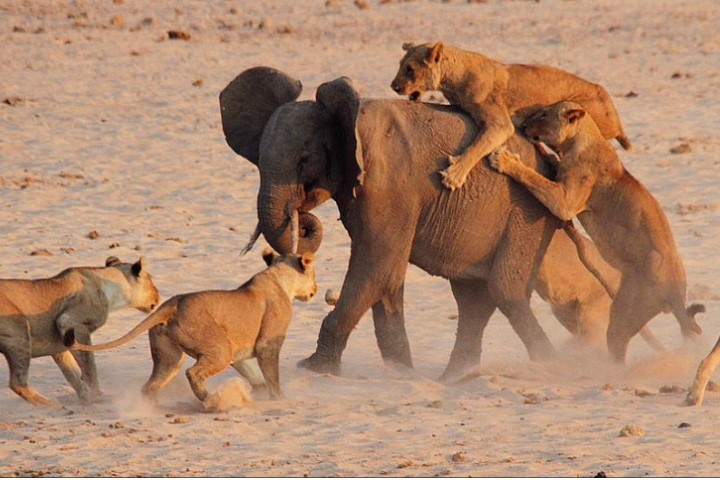
\includegraphics[height=4.5cm]{lion.jpg}
      \caption{狮群的协作捕食}
      \label{fig:lion}
    \end{minipage}\hfill
    \begin{minipage}{0.48\textwidth}
      \centering
      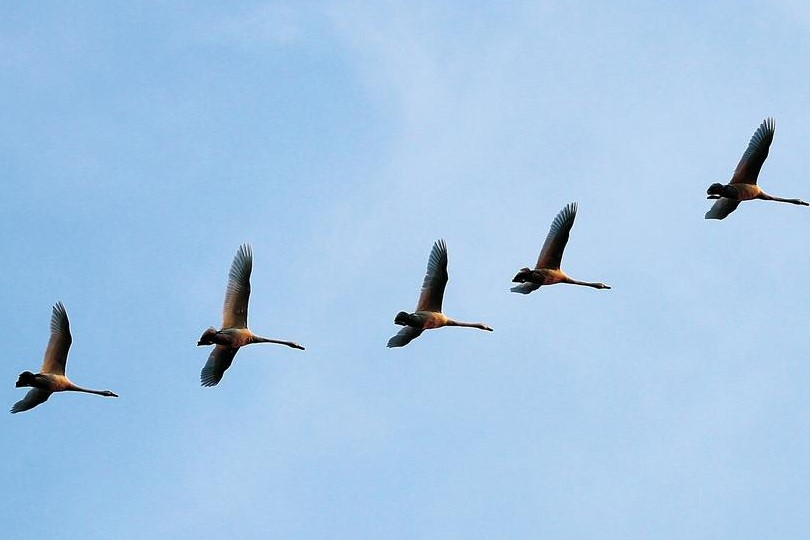
\includegraphics[height=4.5cm]{dayan.jpeg}
      \caption{大雁的成行飞行}
      \label{fig:dayan}
    \end{minipage}
  \end{figure}

在人类生产生活中,也常有协作完成任务的场景,例如车辆编队\cite{ren2008distributed}、分布式传感\cite{lesser2003distributed}、机器人协作\cite{ismail2018survey}等。
人们越来越认识到,相比单个强大而复杂的个体,多个简单个体的合作往往能以更小的代价完成任务。
因此,多智能体系统(\textbf{Multi-Agent Systems, MASs})这一理论模型从自然科学、工程学中抽象出来,引起了越来越多研究者的兴趣。
构成系统的每个智能体具有自己的运行逻辑,从环境中或从其他智能体处获得信息,并作出相应的变化。
智能体之间的信息交互通常受限,且具有独特的交互方式。
智能体各自的运行逻辑,也称作动力学,往往也是复杂而多样。
为了在诸多限制中控制多智能体系统合作完成任务,多智能体协同控制这一子领域应运而生。

多智能体协同控制主要的研究目标有:1.设计分布式的控制协议,仅利用每个智能体从其他智能体处获得的少量信息,进行协同行动;
2.针对各种各类复杂的限制条件,例如故障、攻击、通讯间隔、通讯延迟等,进一步研究并提升控制协议的抗扰性、鲁棒性;
3.探寻协作合作与隐私保护之间的平衡。
多智能体协同控制的研究结合了网络科学、控制科学、计算机科学、数学等多个领域,
需要用到图论、矩阵理论、优化理论等多方面的知识,具有很强的交叉性。

多刚体系统是一类特殊的多智能体系统,系统中的每个智能体为刚体模型,其运行逻辑服从刚体动力学。
刚体是一种理想模型,在外力作用下不会发生形变,刚体的运动包含平动与转动。
飞机、船舶、航天器等人类生产生活中的大量装置均可抽象为刚体模型,因此对多刚体系统的研究,可以应用到这些装置的编队与协作实践中。

近年来无人机集群吸引了人们大量目光,其中用到的不仅仅有无人机的位置协同控制,
还包含了姿态控制,以保证在狭窄严酷的环境中仍能保持编队。
由于小型航天器的发展与发射成本的降低,航天器的编队协作具有广泛的应用与发展前景\cite{long2021distributed}\cite{jin2023synchronization},
一组小型的卫星能以更小的总成本完成一颗大型卫星所不能完成的任务,
例如天基红外干涉阵列、分布式深空观测等,这些应用要求各个航天器姿态一致(或特定朝向)。
从以上两个例子可以看出,刚体模型相比质点模型多出的三个转动自由度增加了刚体的灵活性,
也赋予了多刚体系统完成更加复杂任务的能力,因此多刚体系统姿态控制是多刚体系统实现功能的重要一环。
\begin{figure}[!htp]
    \centering
    \begin{minipage}{0.48\textwidth}
      \centering
      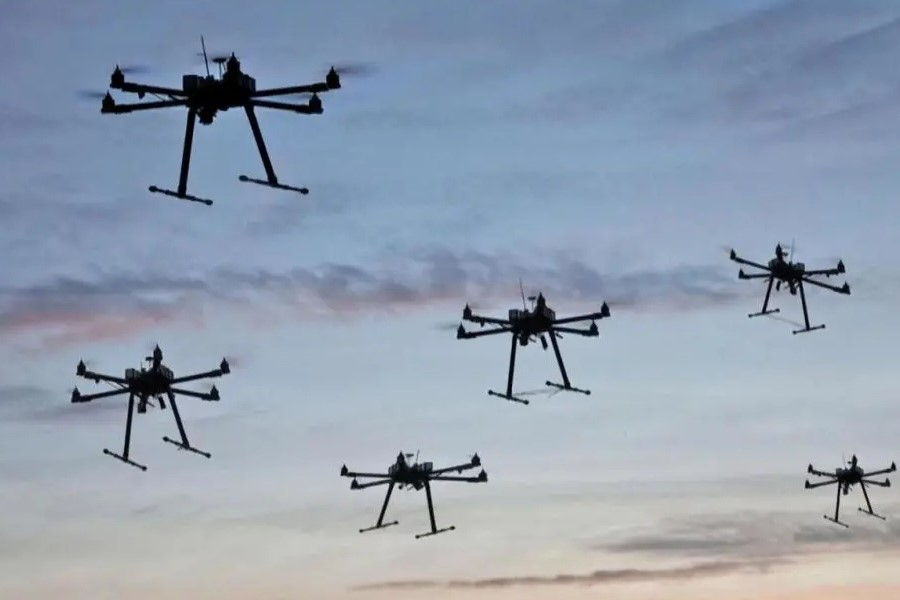
\includegraphics[height=4.5cm]{uav.jpg}
      \caption{无人机集群}
      \label{fig:uav}
    \end{minipage}\hfill
    \begin{minipage}{0.48\textwidth}
      \centering
      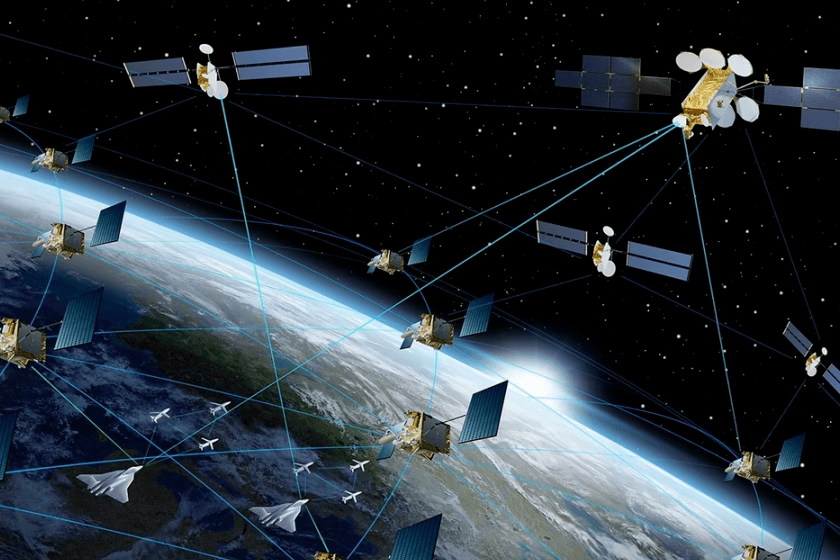
\includegraphics[height=4.5cm]{satellite.png}
      \caption{航天器编队示意图}
      \label{fig:satellite}
    \end{minipage}
  \end{figure}

三个转动自由度的引入,同时也增加了对多刚体系统协同控制研究的挑战性。
姿态(旋转)的变化规律并不是线性的,举一个简单的例子。
先绕$x$轴旋转$\pi/3$再绕$y$轴旋转$\pi/4$得到的姿态,与先绕$y$轴旋转$\pi/4$再绕$x$轴旋转$\pi/3$得到的姿态不相同,
这意味着交换律在姿态问题上是不存在的,因此,我们也不能对姿态求平均值。
这样的数学特性源于旋转空间是一个李群$\text{SO(3)}$\cite{sola2018micro},对加法不封闭,
所以许多处理线性问题的数学方法在姿态系统控制问题上不能使用,需要引入其他的数学工具。
为此,研究者们使用了各种参数来描述旋转,借用微分几何中的定理辅助分析。
相比位置控制,姿态控制是刚体控制研究中更具特色且难度更大的部分,因此本文研究聚焦于多刚体系统姿态协同控制。

总之,多刚体系统姿态协同控制是一个具有广泛应用前景和重要科学意义的问题。
一方面,海、空、天等多层次、多样化的人造装置都具有协作完成任务的需要,多智能体系统理论的一些研究已经广泛应用于各种场景,
而多刚体系统姿态协同控制能为更复杂的任务提供高效的控制策略。
另一方面,针对姿态控制这一非线性控制问题的研究,可以为控制理论非线性问题的处理带来新的理论和方法,
也能为微分几何中的动力学问题提供新的思路。

\section{多刚体姿态一致性的研究现状}

\section{本文研究动机}
\section{本文研究内容和章节安排}

% !TEX root = ../main.tex

\chapter{预备知识}
多刚体系统是一种特殊的多智能体系统,因此在本文接下来的分析计算中,不仅需要用到多智能体系统研究中常用的图论知识、矩阵知识,还需要用到刚体姿态动力学的相关知识。
\section{图论知识}
多刚体系统之间的信息交互网络可以用拓扑图$\mathcal{G}=\{\mathcal{V},\mathcal{E}\}$描述\cite{ren2008distributed}。
$\mathcal{V}=\{1,2,...,n\}$是图的点集,代表系统中的各个刚体,其中$n$为刚体个数。
$\mathcal{E}\subset\mathcal{V}\times\mathcal{V}$是图的边集,其中每个元素(边)是点集中元素的有序对。
边$(i,j)\in\mathcal{E}$代表刚体$j$能获得刚体$i$的信息,此时$i$称为$j$的邻居,或者称$i$为父(首)节点,$j$为子(尾)节点。
点$i$的相邻节点集合为$\mathcal{N}_i=\{j\in\mathcal{V}|(j,i)\in\mathcal{E}\}$,代表所有能让刚体$i$接收到信息的其他刚体。
当$\mathcal{G}$为无向图时,若边$(i,j)\in\mathcal{E}$,则边$(j,i)\in\mathcal{E}$,也就是说刚体之间的通信是相互的,且两者互为邻居。
首尾相连但不形成环的边的集合称为路径,例如$\{(i_1,i_2),(i_2,i_3),...,(i_{m-1},i_m)\}$。
若无向图$\mathcal{G}$中两个点之间都有至少一条路径将它们相连,则称$\mathcal{G}$为连通图。
若无向图$\mathcal{G}$中的任意两个点之间有且仅有一条路径将它们相连,则把$\mathcal{G}$称为树。

除了用集合描述图,还能用矩阵刻画图的性质。图$\mathcal{G}$可以用邻接矩阵$\mathcal{A}$来描述,$\mathcal{A}=[a_{ij}]_{n\times n}$。
若边$(j,i)$存在边集中,即刚体$i$能收到刚体$j$的信息,则$a_{ij}>0$;若边$(j,i)$不存在边集中,即刚体$i$不能收到刚体$j$的信息,则$a_{ij}=0$。
$a_{ij}$的大小代表边的权重,对于平衡图,所有非零的$a_{ij}$设置为$1$,或其他相同的值。
对于节点$i$,所有从$i$出发的边的权重之和称为$i$的出度$d^i_{out}$,$d^i_{out}=\sum_{j=1}^na_{ji}$;
所有到达$i$的边的权重之和称为$i$的入度$d_{in}^i$,$d_{in}^i=\sum_{j=1}^na_{ij}$。
当$\mathcal{G}$为无向图时,邻接矩阵$\mathcal{A}$为对称矩阵,每个节点的入度等于出度。
图$\mathcal{G}$的入读矩阵定义为$\mathcal{D}=\text{diag}(d_{in}^1,d_{in}^2,...,d_{in}^n)$。
图$\mathcal{G}$的拉普拉斯矩阵定义为$\mathcal{L}=[l_{ij}]_{n\times n}=\mathcal{D}-\mathcal{A}$。或者写成
\begin{equation}
    l_{ii}=\sum_{j=1,j\not=i}^n a_{ij},\quad l_{ij}=-a_{ij},i\not=j
\end{equation}
关于$\mathcal{L}$和$x=[x_1^T,x_2^T,...,x_n^T]^T$(每个$x_i$都是$m$维度的向量)通常有以下等式:
\begin{equation}
    \sum{j=1}^na_{ij}(x_i-x_j)=(\mathcal{L}_i\otimes I_m)x
\end{equation}
\begin{equation}
    \sum_{i=1}^n\sum_{j=1}^na_{ij}x_i^T(x_i-x_j)=x^T(\mathcal{L}\otimes I_m)x
\end{equation}
其中$\mathcal{L}_i$表示矩阵$\mathcal{L}$的第$i$行。
定义图$\mathcal{G}$的关联矩阵为$Q=[q_{ik}]\in\mathbb{R}^{n\times p}$,
其中$p$为边集$\mathcal{E}$中元素的个数。
若某条边$e_k$从节点$i$出发到节点$j$终止,则$q_{ik}=1$,$q_{jk}=-1$,第$k$列的其余各元素为0。
关于关联矩阵$Q$,有引理如下
\begin{lemma}
    \label{lm:incidence}
    若无向图$\mathcal{G}$是一棵树,则关联矩阵$Q$满秩。
\end{lemma}
\section{矩阵知识}
\begin{definition}\cite{ren2008distributed}
    对于给定矩阵$A=[a_{ij}]\in\mathbb{R}^{p\times q}$,$B=[b_{ij}]\in\mathbb{R}^{m\times n}$,它们的Kronecker积为
    \begin{equation}
        A\otimes B=\left[\begin{matrix} a_{11}B&\cdots&a_{1q}B\\\vdots&\ddots&\vdots\\a_{p1}B&\cdots&a_{pq}B\end{matrix}\right]\in\mathbb{R}^{pm\times qn}
    \end{equation}
\end{definition}
\begin{lemma}
    对于相同维度的方阵$A$,$B$,$C$,关于矩阵的迹(trace),有如下事实
    \begin{equation}
        \text{tr}(AB)=\text{tr}(BA)
    \end{equation}
    \begin{equation}
        \text{tr}(ABC)=\text{tr}(BCA)=\text{tr}(CAB)
    \end{equation}
\end{lemma}
\begin{lemma}[杨氏不等式]
    \label{lm:young}
    对$\forall x,y\in\mathbb{R}$,有$\epsilon>0$,$xy<\frac{\epsilon}{2}x^2+\frac{1}{2\epsilon}y^2$。
    
    拓展到向量,对$\forall x,y\in\mathbb{R}^m$,有$\epsilon>0$,$x^Ty<\frac{\epsilon}{2}\parallel x\parallel^2+\frac{1}{2\epsilon}\parallel y\parallel^2$。
    其中$\parallel \cdot \parallel$表示向量的2范数 
\end{lemma}
\begin{lemma}\cite{ren2008distributed}
    \label{eigenL}
    对于有向图$\mathcal{G}$,对应拉普拉斯矩阵$\mathcal{L}$,图$\mathcal{G}$含有有向生成树,当且仅当0是$\mathcal{L}$的单特征值,且$\mathcal{L}$的其他特征值实部均大于0。
    对于无向图$\mathcal{G}$,对应拉普拉斯矩阵$\mathcal{L}$,图$\mathcal{G}$是联通的,当且仅当0是$\mathcal{L}$的单特征值。
\end{lemma}
\section{刚体知识}
刚体的姿态由刚体系$\mathcal{F_B}$相对惯性系$\mathcal{F_I}$的旋转描述,
通常用旋转矩阵$R\in \text{SO(3)}$表示。$\text{SO(3)}$是特殊正交群,$\text{SO(3)}=\{R\in \mathbb{R}^{3\times 3}|\det R =1,RR^T=R^TR=I_3\}$。
同时,旋转也可以用欧拉角$\theta\in(-\pi,\pi]$与欧拉轴$u\in \mathbb{S}^2$表示,这两个量代表刚体系相对惯性系绕$u$逆时针旋转了$\theta$。
旋转矩阵与这两者的关系由罗德里格斯旋转公式\cite{sola2018micro}给出:
\begin{equation}
    R=I+u^\wedge\sin\theta+(u^\wedge)^2(1-\cos\theta)
\end{equation}
也可以表示为指数形式
\begin{equation}
    R=\exp((\theta u)^\wedge)
\end{equation}
以上两式中,$(\cdot)^\wedge$将一个三维向量转换成一个三维方阵,对于向量$x=[x_1,x_2,x_3]^T\in\mathbb{R}^3$
\begin{equation}
    x^\wedge=\left[\begin{matrix} 0&-x_3&x_2\\x_3&0&-x_1\\-x_2&x_1&0\end{matrix}\right]
\end{equation}
与之互为逆运算的$(\cdot)^\vee$将一个对角线上元素全为0的三维方阵转换为一个三维向量
\begin{equation}
    \left(\left[\begin{matrix} 0&-x_3&x_2\\x_3&0&-x_1\\-x_2&x_1&0\end{matrix}\right]\right)^\vee=x=[x_1,x_2,x_3]^T
\end{equation}
值得注意的是,上述三维方阵为反对称矩阵,因此有
\begin{equation}
    \label{eq:fanduichen}
    (x^\wedge)^T=-x^\wedge
\end{equation}

关于旋转矩阵及$(\cdot)^\wedge$$(\cdot)^\vee$运算,先给出如下引理
\begin{lemma}\cite{zou2017rotation}
    \label{lm:trace}
    对于向量$x\in\mathbb{R}^3$ 和矩阵$R\in\text{SO(3)}$,$R$对应的欧拉角$\theta$,如下事实成立
    \begin{equation}
        \text{tr}((x^\wedge R))=-x^T(R-R^T)^\vee
    \end{equation}
    \begin{equation}
        (x^\wedge R+R^Tx^\wedge)^\vee=(\text{tr}(R)I_3-R)x
    \end{equation}
    \begin{equation}
        (Rx)^\wedge=Rx^\wedge R^T
    \end{equation}
    \begin{equation}
        \parallel\frac{(R-R^T)^\vee}{2}\parallel=\cos\frac{\theta}{2}\sqrt{\text{tr}(I_3-R)}
    \end{equation}
    \begin{equation}
        \text{tr}(I_3-R)=2(1-\cos\theta)\in[0,4)
    \end{equation}
    $(R-R^T)^\vee=0$,当且仅当$R=I_3$时成立。
\end{lemma}

对于单个刚体,其姿态动力学满足
\begin{equation}
    \label{eq:dynamic1}
    \dot R=R\omega^\wedge
\end{equation}
\begin{equation}
    \label{eq:dynamic2}
    J\dot \omega=-\omega^\wedge J\omega+\tau
\end{equation}
其中$R\in\text{SO(3)}$是刚体系相对于惯性系的旋转矩阵,$\omega\in\mathbb{R}^3$为刚体角速度,$J\in\mathbb{R}^{3\times 3}$为刚体转动惯量矩阵,$\tau\in\mathbb{R}^3$为加在刚体上的力矩,也就是控制算法需要给出的控制律。
$\omega$、$J$、$\tau$都是在刚体系中给出的,而非惯性系下的。
\section{其他引理}
\begin{lemma}\cite{lin2012new}
    令分段连续函数$\phi(t):\mathbb{R}_{\geq0}\rightarrow\mathbb{R}$满足以下条件

    条件1:$\phi(t)$在任意分段区间$(t_{r_j},t_{r_{j+1}})$内是连续与可导的,并在$t_{r_j}$处发生切换,且$\phi(t)$是在$t_{r_j}$处右连续,右可导,$r\in\mathbb{Z}_{\geq0}$,$j=0,1,...,m_r-1$。

    条件2:$\phi(t)$的导数(右导数)在$t\in[0,+\infty)$是有界的,即对于某个常数$\omega>0$,$|\dot\phi(t)|\leq\omega$在$t\in[0,+\infty)$恒成立。

    条件3:$\lim_{t\rightarrow+\infty}\int_{0}^t\phi(\tau)d\tau$存在且有限。

    可以得到
    \begin{equation}
        \lim_{t\rightarrow\infty}\phi(t)=0
    \end{equation}
\end{lemma}
\section{本章小结}
本章介绍了研究多刚体系统所需的相关数学及物理知识,包括图论知识、矩阵知识、刚体知识,引入了一些在后续证明中需要用到的引理定理。

% !TEX root = ../main.tex

\chapter{连续时间系统下多刚体系统姿态一致性}
\section{引言}
\section{问题描述}
考虑$n$个刚体组成的多刚体系统,每个刚体的姿态动力学服从\ref{eq:dynamic1}\ref{eq:dynamic2},即
\begin{equation}
    \label{eq:dynamic3}
    \dot R_i=R_i\omega_i^\wedge
\end{equation}
\begin{equation}
    J_i\dot\omega_i=-\omega_i^\wedge J_i\omega_i+\tau_I
\end{equation}
其中$R_i\in\text{SO(3)}$是刚体系相对于惯性系的旋转矩阵,$\omega_i\in\mathbb{R}^3$为刚体角速度,
$J_i\in\mathbb{R}^{3\times 3}$为刚体转动惯量矩阵,$\tau_i\in\mathbb{R}^3$为加在刚体上的力矩,也就是控制算法需要给出的控制律。
$\omega_i$、$J_i$、$\tau_i$都是在刚体系中给出的,而非惯性系下的。

在此多刚体系统中,我们假设每个刚体$i$能通过测量获得它与部分其他刚体$j$($a_{ij}>0$)之间的相对信息,
并且还能通过自身配备的传感器获得自身绝对角速度信息$\omega_i$。
在本章第三节有相对角速度测量的情况下,相对信息指的是相对姿态$R_j^TR_i$和相对角速度$\omega_i-R_i^TR_j\omega_j$。
在本章第四届无相对角速度测量的情况下,相对信息指的是仅相对姿态$R_j^TR_i$。

基于以上信息,我们希望为此多刚体系统设计一个协议,使得各刚体姿态达到一致,即$R_i=R_j$,$\forall i,j\in\mathcal{V},i\not=j$。

\section{有相对角速度测量}
此部分相对简单,已有一些研究人员从其他角度出发进行了研究\cite{maadani20226}\cite{sarlette2009autonomous},
但为了本文内容的完整性,我们仍在此处给出控制协议并作分析证明。
为解决上述多刚体系统姿态一致性问题,我们给出以下控制协议:
\begin{equation}
    \label{eq:protocol1}
    \tau_i=-k_1\sum_{j=1}^na_{ij}(R_j^TR_i-R_i^TR_j)^{\vee}-k_2\sum_{j=1}^na_{ij}(\omega_i-R_i^TR_j\omega_j)-k_3\omega_i
\end{equation}
其中$k_1$,$k_2$,$k_3$是三个大于0的常数。

\subsection{一致性分析}
利用Lyapunov稳定性理论,分析多刚体系统\ref{eq:dynamic3}在控制协议\ref{eq:protocol1}下的一致性,得到以下结果。
\begin{theorem}
    考虑多刚体系统\ref{eq:dynamic3}和控制协议\ref{eq:protocol1}。若通讯拓扑图$\mathcal{G}$是一个无向连通图,则
    $\lim_{t\rightarrow\infty}\omega_i=0$,$\lim_{t\rightarrow\infty}\sum_{j=1}^na_{ij}(R_j^TR_i-R_i^TR_j)^\vee=0,\forall i$。
    若$\mathcal{G}$是一棵无向树,则多刚体系统姿态能达到一致,即$R_i=R_j$。
    \begin{proof}
        
        首先计算$\text{tr}(R_j^TR_i)$对时间的导数:
        \begin{equation}
            \begin{aligned}
                \dot{(R_j^TR_i)}&=(R_j\omega_j^\wedge)^TR_i+R_j^TR_i\omega_i^\wedge\\
                &=R_j^TR_i(-R_i^TR_j\omega_j^\wedge R_j^TR_i+\omega_i^\wedge)\\
                &=R_j^TR_i(\omega_i-R_i^TR_j\omega_j)^\wedge\\
                \dot{\text{tr}(R_j^TR_i)}&=\text{tr}(\dot{R_j^TR_i})\\
                &=-(\omega_i-R_i^TR_j\omega_j)^T(R_j^TR_i-R_i^TR_j)^\vee
            \end{aligned}
        \end{equation}
        以上用到了\ref{lm:trace}和\ref{eq:fanduichen}。

        设李雅普诺夫函数为
        \begin{equation}
            V=\frac{k_1}{2}\sum_{i=1}^n \sum_{j=1}^n a_{ij}\text{tr}(I_3-R_j^TR_i)+\frac{1}{2}\sum_{i=1}^n\omega_i^TJ_i\omega_i
        \end{equation}
        将$V$对时间求导得到
        \begin{equation}
            \dot V=\sum_{i=1}^n\sum_{j=1}^n\frac{k_1}{2}a_{ij}(\omega_i-R_i^TR_j\omega_j)^T(R_j^TR_i-R_i^TR_j)^\vee+\sum_{i=1}^n\omega_i^TJ_i\dot\omega_i
        \end{equation}
        其中第一项可以写成
        \begin{equation}
            \dot V_1=\sum_{i=1}^n\sum_{j=1}^n\frac{k_1}{2}a_{ij}\omega_i^T(R_j^TR_i-R_i^TR_j)^\vee-\sum_{i=1}^n\sum_{j=1}^n\frac{k_1}{2}a_{ij}(R_i^TR_j\omega_j)^T(R_j^TR_i-R_i^TR_j)^\vee
        \end{equation}

        由\ref{lm:trace},对于旋转矩阵$A\in\text{SO(3)}$和三维列向量$x$,有
        \begin{equation}
            (Ax)^T(A^T-A)^\vee=\text{tr}((Ax)^\wedge A)=\text{tr}(Ax^\wedge A^TA)=\text{tr}(Ax^\wedge)=-x^T(A-A^T)
        \end{equation}
        因此将$\dot V_1$进一步化简得到
        \begin{equation}
            \dot V_1=\sum_{i=1}^n\sum_{j=1}^n\frac{k_1}{2}a_{ij}\omega_i^T(R_j^TR_i-R_i^TR_j)^\vee+\sum_{i=1}^n\sum_{j=1}^n\frac{k_1}{2}a_{ij}\omega_j^T(R_i^TR_j-R_j^TR_i)^\vee
        \end{equation}
        
        由于拓扑图为无向图,$a_{ij}=a_{ji}$,故
        \begin{equation}
            \begin{aligned}
                \dot V_1&=\sum_{i=1}^n\sum_{j=1}^n\frac{k_1}{2}a_{ij}\omega_i^T(R_j^TR_i-R_i^TR_j)^\vee+\sum_{i=1}^n\sum_{j=1}^n\frac{k_1}{2}a_{ji}\omega_j^T(R_i^TR_j-R_j^TR_i)^\vee\\
                &=\sum_{i=1}^n\sum_{j=1}^n\frac{k_1}{2}a_{ij}\omega_i^T(R_j^TR_i-R_i^TR_j)^\vee+\sum_{j=1}^n\sum_{i=1}^n\frac{k_1}{2}a_{ji}\omega_j^T(R_i^TR_j-R_j^TR_i)^\vee\\
                &=\sum_{i=1}^n\sum_{j=1}^nk_1a_{ij}\omega_i^T(R_j^TR_i-R_i^TR_j)^\vee
                \end{aligned}
        \end{equation}
        
        将$\dot V_1$与控制协议\ref{eq:protocol1}代入得到
        \begin{equation}
            \begin{aligned}
                \dot V&=\sum_{i=1}^n\sum_{j=1}^nk_1a_{ij}\omega_i^T(R_j^TR_i-R_i^TR_j)^\vee+\sum_{i=1}^n\omega_i^T(-\omega_i\times J_i\omega_i+\tau_i)\\
                &=\sum_{i=1}^n\sum_{j=1}^nk_1a_{ij}\omega_i^T(R_j^TR_i-R_i^TR_j)^\vee+\sum_{i=1}^n\omega_i^T(-k_1\sum_{j=1}^na_{ij}(R_j^TR_i-R_i^TR_j)^{\vee}\\
                &-k_2\sum_{j=1}^na_{ij}(\omega_i-R_i^TR_j\omega_j)-k_3\omega_i)\\
                &=-k_2\sum_{i=1}^n\sum_{j=1}^n\omega_i^T(\omega_i-R_i^TR_j\omega_j)-\sum_{i=1}^nk_3\omega_i^T\omega_i\\
                &=k_2\sum_{i=1}^n\sum_{j=1}^n(R_i\omega_i)^T(R_i\omega_i-R_j\omega_j)-\sum_{i=1}^nk_3\omega_i^T\omega_i
                \end{aligned}
        \end{equation}
        其中用到了$\omega_i^T(\omega^\wedge J_i\omega_i)=0$。令$R_i\omega_i=\Omega_i$,$\Omega=[\Omega_1^T,\Omega_2^T,...,\Omega_n^T]^T$
        \begin{equation}
            \dot V=-k_2\Omega^T(\mathcal{L}\otimes I_3)\Omega-\sum_{i=1}^nk_3\omega_i^T\omega_i\leq0
        \end{equation}

        令不变集为$\{R_j^TR_i-I_3,\omega_i|\dot V=0\}$。当$\dot V\equiv0$时,$\omega_i\equiv0$,
        由动力学方程\ref{eq:dynamic3}可以得到$\tau_i\equiv0$,代入控制协议\ref{eq:protocol1}得
        \begin{equation}
            \label{eq:equillibrium}
            \sum_{j=1}^na_{ij}(R_j^TR_i-R_i^TR_j)^\vee=0,\quad \forall i
        \end{equation}

        当通讯拓扑图$\mathcal{G}$是一棵无向树时,边集$\mathcal{E}$中的元素个数为$n-1$。
        不妨令$i<j$,令$\hat q\in\mathbb{R}^{3(n-1)}$为所有向量$(R_j^TR_i-R_i^TR_j)^\vee$的组合,$(i,j)\in\mathcal{E}$。
        注意到$(R_j^TR_i-R_i^TR_j)^\vee=-(R_i^TR_j-R_j^TR_i)^\vee$,\ref{eq:equillibrium}可以写成
        \begin{equation}
            (Q\otimes I_3)\hat q=0
        \end{equation}
        其中$Q\in\mathbb{R}^{n\times(n-1)}$,是通讯拓扑图$\mathcal{G}$的关联矩阵。
        根据引理\ref{lm:incidence},$\mathcal{G}$是一棵无向树,矩阵$Q$满秩。
        因此$\hat q=0$,即对相邻的$i,j$,$(R_j^TR_i-R_i^TR_j)^\vee=0$,
        根据引理\ref{lm:trace}和图$\mathcal{G}$的连通性,$R_i=R_j,\forall i\not=j$,姿态达成一致。

        证毕。
    \end{proof}
\end{theorem}

此处姿态一致性的达成有赖于图$\mathcal{G}$是一棵树这一特殊性质,仅依靠$\sum_{j=1}^na_{ij}(R_j^TR_i-R_i^TR_j)^\vee=0,\quad \forall i$这一结果无法得出一致性的结论。
事实上,从仿真结果来看,图$\mathcal{G}$是否是树并不影响一致性,只要图是连通的,姿态一致性都能达成。
关于这一问题,将在本章第六部分进行讨论分析。


\section{无相对角速度测量}
\section{仿真验证}
\section{关于平衡点的讨论}
\section{本章小结}
% !TEX root = ../main.tex

\chapter{简介}

这是 SJTUThesis 的示例文档,基本上覆盖了模板中所有格式的设置。建议大家在使用模
板之前,除了阅读《SJTUThesis 使用文档》,这个示例文档也最好能看一看。

\section{二级标题}

\subsection{三级标题}

\subsubsection{四级标题}

Lorem ipsum dolor sit amet, consectetur adipiscing elit, sed do eiusmod tempor
incididunt ut labore et dolore magna aliqua. Ut enim ad minim veniam, quis
nostrud exercitation ullamco laboris nisi ut aliquip ex ea commodo consequat.
Duis aute irure dolor in reprehenderit in voluptate velit esse cillum dolore eu
fugiat nulla pariatur. Excepteur sint occaecat cupidatat non proident, sunt in
culpa qui officia deserunt mollit anim id est laborum.

\section{脚注}

Lorem ipsum dolor sit amet, consectetur adipiscing elit, sed do eiusmod tempor
incididunt ut labore et dolore magna aliqua. \footnote{Ut enim ad minim veniam,
quis nostrud exercitation ullamco laboris nisi ut aliquip ex ea commodo
consequat. Duis aute irure dolor in reprehenderit in voluptate velit esse cillum
dolore eu fugiat nulla pariatur.}

\section{字体}


上海交通大学是我国历史最悠久的高等学府之一,是教育部直属、教育部与上海市共建的全
国重点大学,是国家“七五”、“八五”重点建设和“211 工程”、“985 工程”的首批建
设高校。经过 115 年的不懈努力,上海交通大学已经成为一所“综合性、研究型、国际化”
的国内一流、国际知名大学,并正在向世界一流大学稳步迈进。 

{\songti 十九世纪末,甲午战败,民族危难。中国近代著名实业家、教育家盛宣怀和一批
  有识之士秉持“自强首在储才,储才必先兴学”的信念,于 1896 年在上海创办了交通大
  学的前身——南洋公学。建校伊始,学校即坚持“求实学,务实业”的宗旨,以培养“第
  一等人才”为教育目标,精勤进取,笃行不倦,在二十世纪二三十年代已成为国内著名的
  高等学府,被誉为“东方MIT”。抗战时期,广大师生历尽艰难,移转租界,内迁重庆,
  坚持办学,不少学生投笔从戎,浴血沙场。解放前夕,广大师生积极投身民主革命,学校
  被誉为“民主堡垒”。
  
  新中国成立初期,为配合国家经济建设的需要,学校调整出相当一部分优势专业、师资设
  备,支持国内兄弟院校的发展。五十年代中期,学校又响应国家建设大西北的号召,根据
  国务院决定,部分迁往西安,分为交通大学上海部分和西安部分。1959 年 3月两部分同
  时被列为全国重点大学,7 月经国务院批准分别独立建制,交通大学上海部分启用“上海
  交通大学”校名。历经西迁、两地办学、独立办学等变迁,为构建新中国的高等教育体
  系,促进社会主义建设做出了重要贡献。六七十年代,学校先后归属国防科工委和六机部
  领导,积极投身国防人才培养和国防科研,为“两弹一星”和国防现代化做出了巨大贡
  献。}

{\heiti 改革开放以来,学校以“敢为天下先”的精神,大胆推进改革:率先组成教授代
  表团访问美国,率先实行校内管理体制改革,率先接受海外友人巨资捐赠等,有力地推动
  了学校的教学科研改革。1984 年,邓小平同志亲切接见了学校领导和师生代表,对学校
  的各项改革给予了充分肯定。在国家和上海市的大力支持下,学校以“上水平、创一流”
  为目标,以学科建设为龙头,先后恢复和兴建了理科、管理学科、生命学科、法学和人文
  学科等。1999 年,上海农学院并入;2005 年,与上海第二医科大学强强合并。至此,学
  校完成了综合性大学的学科布局。近年来,通过国家“985 工程”和“211 工程”的建
  设,学校高层次人才日渐汇聚,科研实力快速提升,实现了向研究型大学的转变。与此同
  时,学校通过与美国密西根大学等世界一流大学的合作办学,实施国际化战略取得重要突
  破。1985 年开始闵行校区建设,历经 20 多年,已基本建设成设施完善,环境优美的现
  代化大学校园,并已完成了办学重心向闵行校区的转移。学校现有徐汇、闵行、法华、七
  宝和重庆南路(卢湾)5 个校区,总占地面积 4840 亩。通过一系列的改革和建设,学校
  的各项办学指标大幅度上升,实现了跨越式发展,整体实力显著增强,为建设世界一流大
  学奠定了坚实的基础。}

{\ifcsname fangsong\endcsname\fangsong\else[无 \cs{fangsong} 字体。]\fi 交通大学
  始终把人才培养作为办学的根本任务。一百多年来,学校为国家和社会培养了 20余万各
  类优秀人才,包括一批杰出的政治家、科学家、社会活动家、实业家、工程技术专家和医
  学专家,如江泽民、陆定一、丁关根、汪道涵、钱学森、吴文俊、徐光宪、张光斗、黄炎
  培、邵力子、李叔同、蔡锷、邹韬奋、陈敏章、王振义、陈竺等。在中国科学院、中国工
  程院院士中,有 200 余位交大校友;在国家 23 位“两弹一星”功臣中,有 6 位交大校
  友;在 18 位国家最高科学技术奖获得者中,有 3 位来自交大。交大创造了中国近现代
  发展史上的诸多“第一”:中国最早的内燃机、最早的电机、最早的中文打字机等;新中国
  第一艘万吨轮、第一艘核潜艇、第一艘气垫船、第一艘水翼艇、自主设计的第一代战斗
  机、第一枚运载火箭、第一颗人造卫星、第一例心脏二尖瓣分离术、第一例成功移植同种
  原位肝手术、第一例成功抢救大面积烧伤病人手术等,都凝聚着交大师生和校友的心血智
  慧。改革开放以来,一批年轻的校友已在世界各地、各行各业崭露头角。}

{\ifcsname kaishu\endcsname\kaishu\else[无 \cs{kaishu} 字体。]\fi 截至 2011 年 12
  月 31 日,学校共有 24 个学院 / 直属系(另有继续教育学院、技术学院和国际教育学
  院),19 个直属单位,12 家附属医院,全日制本科生 16802 人、研究生24495 人(其
  中博士研究生 5059 人);有专任教师 2979 名,其中教授 835 名;中国科学院院士 15
  名,中国工程院院士 20 名,中组部“千人计划”49 名,“长江学者”95 名,国家杰出
  青年基金获得者 80 名,国家重点基础研究发展计划(973 计划)首席科学家 24名,国
  家重大科学研究计划首席科学家 9名,国家基金委创新研究群体 6 个,教育部创新团队
  17 个。
  
  学校现有本科专业 68 个,涵盖经济学、法学、文学、理学、工学、农学、医学、管理学
  和艺术等九个学科门类;拥有国家级教学及人才培养基地 7 个,国家级校外实践教育基
  地 5个,国家级实验教学示范中心 5 个,上海市实验教学示范中心 4 个;有国家级教学
  团队 8个,上海市教学团队 15 个;有国家级教学名师 7 人,上海市教学名师 35 人;
  有国家级精品课程 46 门,上海市精品课程 117 门;有国家级双语示范课程 7
  门;2001、2005 和2009 年,作为第一完成单位,共获得国家级教学成果 37 项、上海市
  教学成果 157项。}

% !TEX root = ../main.tex

\chapter{数学与引用文献的标注}

\section{数学}

\subsection{数字和单位}

宏包 \pkg{siunitx} 提供了更好的数字和单位支持:
\begin{itemize}
  \item \num{12345.67890}
  \item \complexnum{1+-2i}
  \item \num{.3e45}
  \item \numproduct{1.654 x 2.34 x 3.430}
  \item \unit{kg.m.s^{-1}}
  \item \unit{\micro\meter} $\unit{\micro\meter}$
  \item \unit{\ohm} $\unit{\ohm}$
  \item \numlist{10;20}
  \item \numlist{10;20;30}
  \item \qtylist{0.13;0.67;0.80}{\milli\metre}
  \item \numrange{10}{20}
  \item \qtyrange{10}{20}{\degreeCelsius}
\end{itemize}

\subsection{数学符号和公式}

按照国标 GB/T 3102.11—1993《物理科学和技术中使用的数学符号》,
微分符号 $\dd$ 应使用直立体。除此之外,数学常数也应使用直立体:
\begin{itemize}
  \item 微分符号 $\dd$:\cs{dd}
  \item 圆周率 $\uppi$:\cs{uppi}
  \item 自然对数的底 $\ee$:\cs{ee}
  \item 虚数单位 $\ii$, $\jj$:\cs{ii} \cs{jj}
\end{itemize}

公式应另起一行居中排版。公式后应注明编号,按章顺序编排,编号右端对齐。
\begin{equation}
  \ee^{\ii\uppi} + 1 = 0,
\end{equation}
\begin{equation}
  \frac{\dd^2 u}{\dd t^2} = \int f(x) \dd x.
\end{equation}

公式末尾是需要添加标点符号的,至于用逗号还是句号,取决于公式下面一句是接着公式说的,还是另起一句。
\begin{equation}
  \frac{2h}{\pi}\int_{0}^{\infty}\frac{\sin\left( \omega\delta \right)}{\omega}
  \cos\left( \omega x \right) \dd\omega = 
  \begin{cases}
    h, & \left| x \right| < \delta, \\
    \frac{h}{2}, & x = \pm \delta, \\
    0, & \left| x \right| > \delta.
  \end{cases}
\end{equation}
公式较长时最好在等号“$=$”处转行。
\begin{align}
    & I (X_3; X_4) - I (X_3; X_4 \mid X_1) - I (X_3; X_4 \mid X_2) \nonumber \\
  = & [I (X_3; X_4) - I (X_3; X_4 \mid X_1)] - I (X_3; X_4 \mid \tilde{X}_2) \\
  = & I (X_1; X_3; X_4) - I (X_3; X_4 \mid \tilde{X}_2).
\end{align}

如果在等号处转行难以实现,也可在 $+$、$-$、$\times$、$\div$ 运算符号处转行,转行
时运算符号仅书写于转行式前,不重复书写。
\begin{multline}
  \frac{1}{2} \Delta (f_{ij} f^{ij}) =
    2 \left(\sum_{i<j} \chi_{ij}(\sigma_{i} - \sigma_{j})^{2}
    + f^{ij} \nabla_{j} \nabla_{i} (\Delta f) \right. \\
  \left. + \nabla_{k} f_{ij} \nabla^{k} f^{ij} +
    f^{ij} f^{k} \left[2\nabla_{i}R_{jk}
    - \nabla_{k} R_{ij} \right] \vphantom{\sum_{i<j}} \right).
\end{multline}

\subsection{定理环境}

示例文件中使用 \pkg{ntheorem} 宏包配置了定理、引理和证明等环境。用户也可以使用
\pkg{amsthm} 宏包。

这里举一个“定理”和“证明”的例子。
\begin{theorem}[留数定理]
\label{thm:res}
  假设 $U$ 是复平面上的一个单连通开子集,$a_1, \ldots, a_n$ 是复平面上有限个点,
  $f$ 是定义在 $U \backslash \{a_1, \ldots, a_n\}$ 上的全纯函数,如果 $\gamma$
  是一条把 $a_1, \ldots, a_n$ 包围起来的可求长曲线,但不经过任何一个 $a_k$,并且
  其起点与终点重合,那么:

  \begin{equation}
    \label{eq:res}
    \oint\limits_\gamma f(z)\, \dd z = 2\uppi \ii \sum_{k=1}^n \operatorname{I}(\gamma, a_k) \operatorname{Res}(f, a_k).
  \end{equation}

  如果 $\gamma$ 是若尔当曲线,那么 $\operatorname{I}(\gamma, a_k) = 1$,因此:

  \begin{equation}
    \label{eq:resthm}
    \oint\limits_\gamma f(z)\, \dd z = 2\uppi \ii \sum_{k=1}^n \operatorname{Res}(f, a_k).
  \end{equation}

  在这里,$\operatorname{Res}(f, a_k)$ 表示 $f$ 在点 $a_k$ 的留数,
  $\operatorname{I}(\gamma, a_k)$ 表示 $\gamma$ 关于点 $a_k$ 的卷绕数。卷绕数是
  一个整数,它描述了曲线 $\gamma$ 绕过点 $a_k$ 的次数。如果 $\gamma$ 依逆时针方
  向绕着 $a_k$ 移动,卷绕数就是一个正数,如果 $\gamma$ 根本不绕过 $a_k$,卷绕数
  就是零。

  定理~\ref{thm:res} 的证明。

  \begin{proof}
    首先,由……

    其次,……

    所以……
  \end{proof}
\end{theorem}

\section{引用文献的标注}

按照教务处的要求,参考文献外观应符合国标 GB/T 7714 的要求。模版使用 \BibLaTeX{}
配合 \pkg{biblatex-gb7714-2015} 样式包%
\footnote{\url{https://www.ctan.org/pkg/biblatex-gb7714-2015}}%
控制参考文献的输出样式,后端采用 \pkg{biber} 管理文献。

请注意 \pkg{biblatex-gb7714-2015} 宏包 2016 年 9 月才加入 CTAN,如果你使用的
\TeX{} 系统版本较旧,可能没有包含 \pkg{biblatex-gb7714-2015} 宏包,需要手动安装。
\BibLaTeX{} 与 \pkg{biblatex-gb7714-2015} 目前在活跃地更新,为避免一些兼容性问
题,推荐使用较新的版本。

正文中引用参考文献时,使用 \verb|\cite{key1,key2,key3...}| 可以产生“上标引用的参
考文献”,如 \cite{Yu2001,Cheng1999,LSC1957}。使用
\verb|\parencite{key1,key2,key3...}| 则可以产生水平引用的参考文献,例如
\parencite{Li1999,Jiang1989,Hopkinson1999}。请看下面的例子,将会穿插使用水平的和
上标的参考文献:普通图书\parencite{Yu2001,Jiang1998},论文集、会议录
\cite{CSTAM1990},科技报告\parencite{WHO1970},学位论文\cite{Zhang1998},专利文
献\parencite{Jiang1989,HBLZ2001},专著中析出的文献\cite{Cheng1999,GBT2659},期刊
中析出的文献\parencite{Li1999,Li2000},报纸中析出的文献\cite{Ding2000}, 电子文献
\parencite{Jiang1999,Christine1998,Xiao2001}。

可以使用 \verb|\nocite{key1,key2,key3...}| 将参考文献条目加入到文献表中但不在正
文中引用。使用 \verb|\nocite{*}| 可以将参考文献数据库中的所有条目加入到文献表
中。
\nocite{Yang1999,Schinstock2000,Wen1990,GBT16159}

% !TeX root = ../main.tex

\chapter{浮动体}

\section{插图}

插图功能是利用 \TeX{} 的特定编译程序提供的机制实现的,不同的编译程序支持不同的图
形方式。有的同学可能听说“\LaTeX{} 只支持 EPS”,事实上这种说法是不准确的。\XeTeX{}
可以很方便地插入 EPS、PDF、PNG、JPEG 格式的图片。

一般图形都是处在浮动环境中。之所以称为浮动是指最终排版效果图形的位置不一定与源文
件中的位置对应,这也是刚使用 \LaTeX{} 同学可能遇到的问题。如果要强制固定浮动图形
的位置,请使用 \pkg{float} 宏包,它提供了 \texttt{[H]} 参数。

\subsection{单个图形}

图要有图题,研究生图题采用中英文对照,并置于图的编号之后,图的编号和图题应置于图
下方的居中位置。引用图应在图题右上角标出文献来源。文中必须有关于本插图的提示,如
“见图~\ref{fig:energy-distrib}”、“如图~\ref{fig:energy-distrib} 所示”等。该页空
白不够排写该图整体时,则可将其后文字部分提前排写,将图移到次页。

\begin{figure}[!htp]
  \centering
  \begin{tikzpicture}
    \begin{axis}[
      width=12cm,
      height=9cm,
      xmin=0, xmax=7,
      xlabel={$r$ (\unit{\milli\metre})},
      ymin=-1000, ymax=11000,
      ylabel={Energy (\unit[per-mode=symbol]{\watt\per\cubic\metre})},
      scaled ticks=false,
      tick label style={
        /pgf/number format/1000 sep=,
        font={\zihao{-5}},
      },
      minor tick num=1,
      tick pos=left,
      tick align=outside,
      tick style={thin,black},
    ]
      \addplot [only marks,mark=square*] 
        table [x={radial}, y={energy}, col sep=comma] 
        {./assets/energy-distrib.csv};
      \node at (2,6000) 
        {$q_{v}=\dfrac{\sigma\omega^{2}|\mathbf{A}|^{2}}{2}$};
    \end{axis}
  \end{tikzpicture}
  \bicaption{内热源沿径向的分布}{Energy distribution along radial}
  \label{fig:energy-distrib}
\end{figure}

\subsection{多个图形}

简单插入多个图形的例子如图~\ref{fig:SRR} 所示。这两个水平并列放置的子图共用一个
图形计数器,没有各自的子图题。

\begin{figure}[!htp]
  \centering
  
\includegraphics[height=2cm]{sjtu-vi-badge-blue.pdf}
  \hspace{1cm}
  
\includegraphics[height=2cm]{sjtu-vi-badge-blue.pdf}
  \bicaption{中文题图}{English caption}
  \label{fig:SRR}
\end{figure}

如果多个图形相互独立,并不共用一个图形计数器,那么用 \texttt{minipage} 或者
\texttt{parbox} 就可以,如图~\ref{fig:parallel1} 与图~\ref{fig:parallel2}。

\begin{figure}[!htp]
  \centering
  \begin{minipage}{0.48\textwidth}
    \centering
    
\includegraphics[height=1.5cm]{sjtu-vi-name-blue.pdf}
    \caption{并排第一个图}
    \label{fig:parallel1}
  \end{minipage}\hfill
  \begin{minipage}{0.48\textwidth}
    \centering
    
\includegraphics[height=1.5cm]{sjtu-vi-name-blue.pdf}
    \caption{并排第二个图}
    \label{fig:parallel2}
  \end{minipage}
\end{figure}

如果要为共用一个计数器的多个子图添加子图题,建议使用较新的 \pkg{subcaption}宏
包,不建议使用 \pkg{subfigure} 或 \pkg{subfig} 等宏包。

推荐使用 \pkg{subcaption} 宏包的 \cs{subcaptionbox} 并排子图,子图题置于子图之
下,子图号用 a)、b) 等表示。也可以使用 \pkg{subcaption} 宏包的 \cs{subcaption}
(放在 minipage中,用法同 \cs{caption})。

\pkg{subcaption} 宏包也提供了 \pkg{subfigure} 和 \pkg{subtable} 环境,如
图~\ref{fig:subfigure}。

\begin{figure}[!htp]
  \centering
  \begin{subfigure}{0.3\textwidth}
    \centering
    
\includegraphics[height=2cm]{sjtu-vi-badge-blue.pdf}
    \caption{校徽}
  \end{subfigure}
  \hspace{1cm}
  \begin{subfigure}{0.4\textwidth}
    \centering
    
\includegraphics[height=1.5cm]{sjtu-vi-name-blue.pdf}
    \caption{校名。注意这个图略矮些,subfigure 中同一行的子图在顶端对齐。}
  \end{subfigure}
  \caption{包含子图题的范例(使用 subfigure)}
  \label{fig:subfigure}
\end{figure}

搭配 \pkg{bicaption} 宏包时,可以启用 \cs{subcaptionbox} 和 \cs{subcaption} 的双
语变种 \cs{bisubcaptionbox} 和 \cs{bisubcaption},如图~\ref{fig:bisubcaptionbox}
所示。

\begin{figure}[!hbtp]
  \centering
  \bisubcaptionbox{$R_3 = 1.5\text{mm}$ 时轴承的压力分布云图}%
                  {Pressure contour of bearing when $R_3 = 1.5\text{mm}$}%
                  [6.4cm]{\includegraphics[height=3cm]{example-image-a.pdf}}
  \hspace{1cm}
  \bisubcaptionbox{$R_3 = 2.5\text{mm}$ 时轴承的压力分布云图}%
                  {Pressure contour of bearing when $R_3 = 2.5\text{mm}$}%
                  [6.4cm]{\includegraphics[height=3cm]{example-image-b.pdf}}
  \bicaption{包含子图题的范例(使用 subcaptionbox)}
            {Example with subcaptionbox}
  \label{fig:bisubcaptionbox}
\end{figure}


\section{表格}

\subsection{基本表格}

编排表格应简单明了,表达一致,明晰易懂,表文呼应、内容一致。表题置于表上,研究生
学位论文可以用中、英文两种文字居中排写,中文在上,也可以只用中文。

表格的编排建议采用国际通行的三线表\footnote{三线表,以其形式简洁、功能分明、阅读
方便而在科技论文中被推荐使用。三线表通常只有 3 条线,即顶线、底线和栏目线,没有
竖线。}。三线表可以使用 \pkg{booktabs} 提供的 \cs{toprule}、\cs{midrule} 和
\cs{bottomrule}。它们与 \pkg{longtable} 能很好的配合使用。

\begin{table}[!hpt]
  \caption[一个颇为标准的三线表]{一个颇为标准的三线表\footnotemark}
  \label{tab:firstone}
  \centering
  \begin{tabular}{@{}llr@{}} \toprule
    \multicolumn{2}{c}{Item} \\ \cmidrule(r){1-2}
    Animal & Description & Price (\$)\\ \midrule
    Gnat  & per gram  & 13.65 \\
          & each      & 0.01 \\
    Gnu   & stuffed   & 92.50 \\
    Emu   & stuffed   & 33.33 \\
    Armadillo & frozen & 8.99 \\ \bottomrule
  \end{tabular}
\end{table}
\footnotetext{这个例子来自
  \href{https://mirrors.sjtug.sjtu.edu.cn/ctan/macros/latex/contrib/booktabs/booktabs.pdf}%
  {《Publication quality tables in LaTeX》}(\pkg{booktabs} 宏包的文档)。这也是
  一个在表格中使用脚注的例子,请留意与 \pkg{threeparttable} 实现的效果有何不
  同。}

\subsection{复杂表格}

我们经常会在表格下方标注数据来源,或者对表格里面的条目进行解释。可以用
\pkg{threeparttable} 实现带有脚注的表格,如表~\ref{tab:footnote}。

\begin{table}[!htpb]
  \bicaption{一个带有脚注的表格的例子}{A Table with footnotes}
  \label{tab:footnote}
  \centering
  \begin{threeparttable}[b]
     \begin{tabular}{ccd{4}cccc}
      \toprule
      \multirow{2}*{total} & \multicolumn{2}{c}{20\tnote{a}} & \multicolumn{2}{c}{40} & \multicolumn{2}{c}{60} \\
      \cmidrule(lr){2-3}\cmidrule(lr){4-5}\cmidrule(lr){6-7}
      & www & \multicolumn{1}{c}{k} & www & k & www & k \\ % 使用说明符 d 的列会自动进入数学模式,使用 \multicolumn 对文字表头做特殊处理
      \midrule
      & $\underset{(2.12)}{4.22}$ & 120.0140\tnote{b} & 333.15 & 0.0411 & 444.99 & 0.1387 \\
      & 168.6123 & 10.86 & 255.37 & 0.0353 & 376.14 & 0.1058 \\
      & 6.761    & 0.007 & 235.37 & 0.0267 & 348.66 & 0.1010 \\
      \bottomrule
    \end{tabular}
    \begin{tablenotes}
    \item [a] the first note.
    \item [b] the second note.
    \end{tablenotes}
  \end{threeparttable}
\end{table}

如某个表需要转页接排,可以用 \pkg{longtable} 实现。接排时表题省略,表头应重复书
写,并在右上方写“续表 xx”,如表~\ref{tab:performance}。

\begin{ThreePartTable}
  \begin{TableNotes}
    \item[a] 一个脚注
    \item[b] 另一个脚注
  \end{TableNotes}
  \begin{longtable}[c]{c*{6}{r}}
    \bicaption{实验数据}{Experimental data}
    \label{tab:performance} \\
    \toprule
    测试程序 & \multicolumn{1}{c}{正常运行} & \multicolumn{1}{c}{同步}
      & \multicolumn{1}{c}{检查点} & \multicolumn{1}{c}{卷回恢复}
      & \multicolumn{1}{c}{进程迁移} & \multicolumn{1}{c}{检查点} \\
    & \multicolumn{1}{c}{时间 (s)} & \multicolumn{1}{c}{时间 (s)}
      & \multicolumn{1}{c}{时间 (s)} & \multicolumn{1}{c}{时间 (s)}
      & \multicolumn{1}{c}{时间 (s)} &  文件(KB)\\
    \midrule
    \endfirsthead
    \multicolumn{7}{l}{\textbf{续表~\thetable}} \\
    % 英语论文:\multicolumn{7}{r}{\textbf{Table~\thetable~(continued)}} \\
    \toprule
    测试程序 & \multicolumn{1}{c}{正常运行} & \multicolumn{1}{c}{同步}
      & \multicolumn{1}{c}{检查点} & \multicolumn{1}{c}{卷回恢复}
      & \multicolumn{1}{c}{进程迁移} & \multicolumn{1}{c}{检查点} \\
    & \multicolumn{1}{c}{时间 (s)} & \multicolumn{1}{c}{时间 (s)}
      & \multicolumn{1}{c}{时间 (s)} & \multicolumn{1}{c}{时间 (s)}
      & \multicolumn{1}{c}{时间 (s)}&  文件(KB)\\
    \midrule
    \endhead
    \hline
    \multicolumn{7}{r}{续下页}
    \endfoot
    \insertTableNotes
    \endlastfoot
    CG.A.2 & 23.05 & 0.002 & 0.116 & 0.035 & 0.589 & 32491 \\
    CG.A.4 & 15.06 & 0.003 & 0.067 & 0.021 & 0.351 & 18211 \\
    CG.A.8 & 13.38 & 0.004 & 0.072 & 0.023 & 0.210 & 9890 \\
    CG.B.2 & 867.45 & 0.002 & 0.864 & 0.232 & 3.256 & 228562 \\
    CG.B.4 & 501.61 & 0.003 & 0.438 & 0.136 & 2.075 & 123862 \\
    CG.B.8 & 384.65 & 0.004 & 0.457 & 0.108 & 1.235 & 63777 \\
    MG.A.2 & 112.27 & 0.002 & 0.846 & 0.237 & 3.930 & 236473 \\
    MG.A.4 & 59.84 & 0.003 & 0.442 & 0.128 & 2.070 & 123875 \\
    MG.A.8 & 31.38 & 0.003 & 0.476 & 0.114 & 1.041 & 60627 \\
    MG.B.2 & 526.28 & 0.002 & 0.821 & 0.238 & 4.176 & 236635 \\
    MG.B.4 & 280.11 & 0.003 & 0.432 & 0.130 & 1.706 & 123793 \\
    MG.B.8 & 148.29 & 0.003 & 0.442 & 0.116 & 0.893 & 60600 \\
    LU.A.2 & 2116.54 & 0.002 & 0.110 & 0.030 & 0.532 & 28754 \\
    LU.A.4 & 1102.50 & 0.002 & 0.069 & 0.017 & 0.255 & 14915 \\
    LU.A.8 & 574.47 & 0.003 & 0.067 & 0.016 & 0.192 & 8655 \\
    LU.B.2 & 9712.87 & 0.002 & 0.357 & 0.104 & 1.734 & 101975 \\
    LU.B.4 & 4757.80 & 0.003 & 0.190 & 0.056 & 0.808 & 53522 \\
    LU.B.8 & 2444.05 & 0.004 & 0.222 & 0.057 & 0.548 & 30134 \\
    EP.A.2 & 123.81 & 0.002 & 0.010 & 0.003 & 0.074 & 1834 \\
    EP.A.4 & 61.92 & 0.003 & 0.011 & 0.004 & 0.073 & 1743 \\
    EP.A.8 & 31.06 & 0.004 & 0.017 & 0.005 & 0.073 & 1661 \\
    EP.B.2 & 495.49 & 0.001 & 0.009 & 0.003 & 0.196 & 2011 \\
    EP.B.4 & 247.69 & 0.002 & 0.012 & 0.004 & 0.122 & 1663 \\
    EP.B.8 & 126.74 & 0.003 & 0.017 & 0.005 & 0.083 & 1656 \\
    SP.A.2 & 123.81 & 0.002 & 0.010 & 0.003 & 0.074 & 1854 \\
    SP.A.4 & 51.92 & 0.003 & 0.011 & 0.004 & 0.073 & 1543 \\
    SP.A.8 & 31.06 & 0.004 & 0.017 & 0.005 & 0.073 & 1671 \\
    SP.B.2 & 495.49 & 0.001 & 0.009 & 0.003 & 0.196 & 2411 \\
    SP.B.4 \tnote{a} & 247.69 & 0.002 & 0.014 & 0.006 & 0.152 & 2653 \\
    SP.B.8 \tnote{b} & 126.74 & 0.003 & 0.017 & 0.005 & 0.082 & 1755 \\
    \bottomrule
  \end{longtable}
\end{ThreePartTable}

\section{算法环境}

算法环境可以使用 \pkg{algorithms} 宏包或者较新的 \pkg{algorithm2e} 实现。
算法~\ref{algo:algorithm} 是一个使用 \pkg{algorithm2e} 的例子。关于排版算法环境
的具体方法,请阅读相关宏包的官方文档。

\begin{algorithm}[htb]
  \caption{算法示例}
  \label{algo:algorithm}
  \small
  \SetAlgoLined
  \KwData{this text}
  \KwResult{how to write algorithm with \LaTeXe }

  initialization\;
  \While{not at end of this document}{
    read current\;
    \eIf{understand}{
      go to next section\;
      current section becomes this one\;
    }{
      go back to the beginning of current section\;
    }
  }
\end{algorithm}

\section{代码环境}

我们可以在论文中插入算法,但是不建议插入大段的代码。如果确实需要插入代码,建议使
用 \pkg{listings} 宏包。

\begin{codeblock}[language=C]
#include <stdio.h>
#include <unistd.h>
#include <sys/types.h>
#include <sys/wait.h>

int main() {
  pid_t pid;

  switch ((pid = fork())) {
  case -1:
    printf("fork failed\n");
    break;
  case 0:
    /* child calls exec */
    execl("/bin/ls", "ls", "-l", (char*)0);
    printf("execl failed\n");
    break;
  default:
    /* parent uses wait to suspend execution until child finishes */
    wait((int*)0);
    printf("is completed\n");
    break;
  }

  return 0;
}
\end{codeblock}

% !TEX root = ../main.tex

\chapter{全文总结}

这里是全文总结内容。

2015 年 2 月 28 日,中央在北京召开全国精神文明建设工作表彰暨学雷锋志愿服务大会,
公布全国文明城市(区)、文明村镇、文明单位名单。上海交通大学荣获全国文明单位称
号。

全国文明单位这一荣誉是对交大人始终高度重视文明文化工作的肯定,是对交大长期以来文
明创建工作成绩的褒奖。在学校党委、文明委的领导下,交大坚持将文明创建工作纳入学校
建设世界一流大学的工作中,全体师生医护员工群策群力、积极开拓,落实国家和上海市有
关文明创建的各项要求,以改革创新、科学发展为主线,以质量提升为目标,聚焦文明创建
工作出现的重点和难点,优化文明创建工作机制,传播学校良好形象,提升社会美誉度,显
著增强学校软实力。2007 至 2012 年间,上海交大连续三届荣获“上海市文明单位”称
号,成为创建全国文明单位的新起点。

上海交大自启动争创全国文明单位工作以来,凝魂聚气、改革创新,积极培育和践行社会主
义核心价值观。坚持统筹兼顾、多措并举,将争创全国文明单位与学校各项中心工作紧密结
合,着力构建学校文明创建新格局,不断提升师生医护员工文明素养,以“冲击世界一流大
学汇聚强大精神动力”为指导思想,以“聚焦改革、多元推进、以评促建、丰富内涵、彰显
特色”为工作原则,并由全体校领导群策领衔“党的建设深化、思想教育深入、办学成绩显
著、大学文化丰富、校园环境优化、社会责任担当”六大板块共 28 项重点突破工作,全面
展现近年来交大文明创建工作的全貌和成就。

进入新阶段,学校将继续开拓文明创建工作新格局,不断深化工作理念和工作实践,创新工
作载体、丰富活动内涵、凸显创建成效,积极服务于学校各项中心工作和改革发展的大局
面,在上级党委、文明委的关心下,在学校党委的直接领导下,与时俱进、开拓创新,为深
化内涵建设、加快建成世界一流大学、推动国家进步和社会发展而努力奋斗!

上海交通大学医学院附属仁济医院也获得全国文明单位称号。


%TC:ignore

% 参考文献
\printbibliography[heading=bibintoc]

% 附录
\appendix

% 附录中图表不加入索引
\captionsetup{list=no}

% 附录内容
% !TEX root = ../main.tex

\chapter{Maxwell Equations}

选择二维情况,有如下的偏振矢量:
\begin{subequations}
  \begin{align}
    {\bf E} &= E_z(r, \theta) \hat{\bf z}, \\
    {\bf H} &= H_r(r, \theta) \hat{\bf r} + H_\theta(r, \theta) \hat{\bm\theta}.
  \end{align}
\end{subequations}
对上式求旋度:
\begin{subequations}
  \begin{align}
    \nabla \times {\bf E} &= \frac{1}{r} \frac{\partial E_z}{\partial\theta}
      \hat{\bf r} - \frac{\partial E_z}{\partial r} \hat{\bm\theta}, \\
    \nabla \times {\bf H} &= \left[\frac{1}{r} \frac{\partial}{\partial r}
      (r H_\theta) - \frac{1}{r} \frac{\partial H_r}{\partial\theta} \right]
      \hat{\bf z}.
  \end{align}
\end{subequations}
因为在柱坐标系下,$\overline{\overline\mu}$ 是对角的,所以 Maxwell 方程组中电场
$\bf E$ 的旋度:
\begin{subequations}
  \begin{align}
    & \nabla \times {\bf E} = \ii \omega {\bf B}, \\
    & \frac{1}{r} \frac{\partial E_z}{\partial\theta} \hat{\bf r} -
      \frac{\partial E_z}{\partial r}\hat{\bm\theta} = \ii \omega \mu_r H_r
      \hat{\bf r} + \ii \omega \mu_\theta H_\theta \hat{\bm\theta}.
  \end{align}
\end{subequations}
所以 $\bf H$ 的各个分量可以写为:
\begin{subequations}
  \begin{align}
    H_r &= \frac{1}{\ii \omega \mu_r} \frac{1}{r}
      \frac{\partial E_z}{\partial\theta}, \\
    H_\theta &= -\frac{1}{\ii \omega \mu_\theta}
      \frac{\partial E_z}{\partial r}.
  \end{align}
\end{subequations}
同样地,在柱坐标系下,$\overline{\overline\epsilon}$ 是对角的,所以 Maxwell 方程
组中磁场 $\bf H$ 的旋度:
\begin{subequations}
  \begin{align}
    & \nabla \times {\bf H} = -\ii \omega {\bf D}, \\
    & \left[\frac{1}{r} \frac{\partial}{\partial r}(r H_\theta) - \frac{1}{r}
      \frac{\partial H_r}{\partial\theta} \right] \hat{\bf z} = -\ii \omega
      {\overline{\overline\epsilon}} {\bf E} = -\ii \omega \epsilon_z E_z
      \hat{\bf z}, \\
    & \frac{1}{r} \frac{\partial}{\partial r}(r H_\theta) - \frac{1}{r}
      \frac{\partial H_r}{\partial\theta} = -\ii \omega \epsilon_z E_z.
  \end{align}
\end{subequations}
由此我们可以得到关于 $E_z$ 的波函数方程:
\begin{equation}
  \frac{1}{\mu_\theta \epsilon_z} \frac{1}{r} \frac{\partial}{\partial r}
  \left(r \frac{\partial E_z}{\partial r} \right) + \frac{1}{\mu_r \epsilon_z}
  \frac{1}{r^2} \frac{\partial^2E_z}{\partial\theta^2} +\omega^2 E_z = 0.
\end{equation}

% !TEX root = ../main.tex

\chapter{绘制流程图}

图~\ref{fig:flow_chart} 是一张流程图示意。使用 \pkg{tikz} 环境,搭配四种预定义节
点(\verb|startstop|、\verb|process|、\verb|decision| 和 \verb|io|),可以容易地
绘制出流程图。

\begin{figure}[!htp]
  \centering
  
% 定义流程图节点
\tikzstyle{startstop} = [
  rectangle,
  rounded corners,
  minimum width=4em,
  text centered,
  inner sep=1.5ex,
  draw
]
\tikzstyle{io} = [
  trapezium,
  trapezium left angle=75,
  trapezium right angle=105,
  minimum width=4em,
  text centered,
  inner sep=1.5ex,
  draw
]
\tikzstyle{process} = [
  rectangle,
  minimum width=4em,
  text centered,
  inner sep=1.5ex,
  draw
]
\tikzstyle{decision} = [
  diamond,
  minimum width=4em,
  aspect=2,
  text centered,
  draw
]
\tikzstyle{arrow} = [-{LaTeX}]

\begin{tikzpicture}[node distance=1.5cm, every node/.style={font=\footnotesize}]
  % 设置节点
  \node[startstop] (pic) {待测图片};
  \node[io, below of=pic] (bg) {读取背景};
  \node[process, below of=bg] (pair) {匹配特征点对};
  \node[decision, below of=pair, yshift=-2ex] (threshold) {多于阈值};
  \node[decision, right of=threshold, xshift=3cm] (clear) {清晰?};
  \node[process, right of=pair, xshift=3cm] (capture) {重采};
  \node[process, below of=threshold, yshift=-2ex] (matrix_p) {透视变换矩阵};
  \node[process, right of=matrix_p, xshift=3cm] (matrix_a) {仿射变换矩阵};
  \node[process, below of=matrix_p] (reg) {图像修正};
  \node[startstop, below of=reg] (return) {配准结果};
    
  % 连接节点
  \draw[arrow] (pic) -- (bg);
  \draw[arrow] (bg) -- (pair);
  \draw[arrow] (pair) -- (threshold);

  \draw[arrow] (threshold) -- node[above] {否} (clear);

  \draw[arrow] (clear) -- node[right] {否} (capture);
  \draw[arrow] (capture) |- (pic);
  \draw[arrow] (clear) -- node[right] {是} (matrix_a);
  \draw[arrow] (matrix_a) |- (reg);

  \draw[arrow] (threshold) -- node[left] {是} (matrix_p);
  \draw[arrow] (matrix_p) -- (reg);
  \draw[arrow] (reg) -- (return);
\end{tikzpicture}

  \bicaption{绘制流程图效果}{Flow chart}
  \label{fig:flow_chart}
\end{figure}


% 结尾部分
\backmatter

% 用于盲审的论文需隐去致谢、发表论文、科研成果、简历

% 致谢
% !TEX root = ../main.tex

\begin{acknowledgements}
  感谢那位最先制作出博士学位论文 \LaTeX{} 模板的物理系同学!

  感谢 William Wang 同学对模板移植做出的贡献!

  感谢 \href{https://github.com/weijianwen}{@weijianwen} 学长开创性的工作!

  感谢 \href{https://github.com/sjtug}{@sjtug} 对 0.10 及之后版本的开发和维护工作!

  感谢所有为模板贡献过代码的\href{https://github.com/sjtug/SJTUThesis/graphs/contributors}{同学们}, 以及所有测试和使用模板的各位同学!

  感谢 \LaTeX 和 \href{https://github.com/sjtug/SJTUThesis}{SJTUThesis},帮我节省了不少时间。
\end{acknowledgements}


% 发表论文及科研成果
% 盲审论文中,发表论文及科研成果等仅以第几作者注明即可,不要出现作者或他人姓名
% !TEX root = ../main.tex

\begin{achievements}

\subsection*{学术论文}

\begin{bibliolist}{00}
  \item Chen H, Chan C~T. Acoustic cloaking in three dimensions using acoustic metamaterials[J]. Applied Physics Letters, 2007, 91:183518.
  \item Chen H, Wu B~I, Zhang B, et al. Electromagnetic Wave Interactions with a Metamaterial Cloak[J]. Physical Review Letters, 2007, 99(6):63903.
\end{bibliolist}

\begin{bibliolist*}{00}
  \item 第一作者. 中文核心期刊论文, 2007.
  \item 第一作者. EI 国际会议论文, 2006.
\end{bibliolist*}

\subsection*{专利}

\begin{bibliolist}{00}
  \item 第一发明人, “永动机”, 专利申请号202510149890.0.
\end{bibliolist}

\begin{bibliolist*}{00}
  \item 第一发明人, “永动机”, 专利申请号XXXXXXXXXXXX.X.
\end{bibliolist*}

\end{achievements}


% 简历
% !TEX root = ../main.tex

\begin{resume}
  \subsection*{基本情况}
    某某,yyyy 年 mm 月生于 xxxx。

  \subsection*{教育背景}
  \begin{itemize}
    \item yyyy 年 mm 月至今,上海交通大学,博士研究生,xx 专业
    \item yyyy 年 mm 月至 yyyy 年 mm 月,上海交通大学,硕士研究生,xx 专业
    \item yyyy 年 mm 月至 yyyy 年 mm 月,上海交通大学,本科,xx 专业
  \end{itemize}

  \subsection*{研究兴趣}
    \LaTeX{} 排版

  \subsection*{联系方式}
  \begin{itemize}
    \item 地址: 上海市闵行区东川路 800 号,200240
    \item E-mail: \email{john_smith@sjtu.edu.cn}
  \end{itemize}
\end{resume}


% 学士学位论文要求在最后有一个大摘要,单独编页码
% !TEX root = ../main.tex

\begin{digest}
  An imperial edict issued in 1896 by Emperor Guangxu, established Nanyang
  Public School in Shanghai. The normal school, school of foreign studies,
  middle school and a high school were established. Sheng Xuanhuai, the person
  responsible for proposing the idea to the emperor, became the first president
  and is regarded as the founder of the university.

  During the 1930s, the university gained a reputation of nurturing top
  engineers. After the foundation of People's Republic, some faculties were
  transferred to other universities. A significant amount of its faculty were
  sent in 1956, by the national government, to Xi'an to help build up Xi'an Jiao
  Tong University in western China. Afterwards, the school was officially
  renamed Shanghai Jiao Tong University.

  Since the reform and opening up policy in China, SJTU has taken the lead in
  management reform of institutions for higher education, regaining its vigor
  and vitality with an unprecedented momentum of growth. SJTU includes five
  beautiful campuses, Xuhui, Minhang, Luwan Qibao, and Fahua, taking up an area
  of about \qty{3225833}{\square\metre}. A number of disciplines have been
  advancing towards the top echelon internationally, and a batch of burgeoning
  branches of learning have taken an important position domestically.

  Today SJTU has 31 schools (departments), 63 undergraduate programs, 250
  masters-degree programs, 203 Ph.D. programs, 28 post-doctorate programs, and
  11 state key laboratories and national engineering research centers.

  SJTU boasts a large number of famous scientists and professors, including 35
  academics of the Academy of Sciences and Academy of Engineering, 95 accredited
  professors and chair professors of the ``Cheung Kong Scholars Program'' and
  more than \num{2000} professors and associate professors.

  Its total enrollment of students amounts to \num{35929}, of which \num{1564}
  are international students. There are \num{16802} undergraduates, and
  \num{17563} masters and Ph.D. candidates. After more than a century of
  operation, Jiao Tong University has inherited the old tradition of ``high
  starting points, solid foundation, strict requirements and extensive
  practice.'' Students from SJTU have won top prizes in various competitions,
  including ACM International Collegiate Programming Contest, International
  Mathematical Contest in Modeling and Electronics Design Contests. Famous
  alumni include Jiang Zemin, Lu Dingyi, Ding Guangen, Wang Daohan, Qian Xuesen,
  Wu Wenjun, Zou Taofen, Mao Yisheng, Cai Er, Huang Yanpei, Shao Lizi, Wang An
  and many more. More than 200 of the academics of the Chinese Academy of
  Sciences and Chinese Academy of Engineering are alumni of Jiao Tong
  University.
\end{digest}


%TC:endignore

\end{document}
